\documentclass[10pt]{article}

\usepackage[margin=1in]{geometry}
\usepackage[T1]{fontenc}
\usepackage[utf8]{inputenc}
\usepackage{booktabs}
\usepackage{amsmath}
\usepackage{graphicx}
\usepackage{float}
\usepackage{hyperref}
\usepackage{microtype}
\usepackage{caption}

\title{Dataset-Dependent Exploration-Exploitation Tradeoffs\\for Ligand-Based Virtual Screening}
\author{Zhiwen Bian \and Enhao He}
\date{}

\begin{document}
\maketitle

\begin{abstract}
This report studies ligand-based virtual screening as an active-molecule recovery problem rather than a classifier-training problem. Under a fixed evaluation budget, the goal is to select molecules that recover active compounds as quickly as possible. We compare pure exploitation, fixed exploration-exploitation mixtures, a simple adaptive alpha strategy, a UCB bandit adaptive alpha strategy, and a cluster-weighted bandit extension across five molecular screening datasets with different observed hit rates: HIV, ClinTox, Tox21, BACE, and BBBP. The results show that pure uncertainty is not a reliable screening objective. Strong strategies are usually exploitative or mildly exploratory, and the preferred exploration weight is dataset-dependent. The bandit adaptive strategy improves substantially over the simple adaptive rule on BACE and Tox21. Cluster-weighted batch diversity improves recall on some sparse or high-prevalence tasks, but can reduce AUSC when diversity pressure overrides hit-seeking.
\end{abstract}

\section{Objective}

Virtual screening is used to prioritize active molecules from large candidate libraries before expensive downstream testing. In this project, the predictive model is not the final objective. Instead, the model is a surrogate used to rank molecules for evaluation. The practical goal is:
\[
\text{recover as many active molecules as possible under a fixed evaluation budget.}
\]
Therefore, acquisition strategies should be evaluated by screening metrics such as active-molecule recall and area under the screening curve (AUSC), not only by classifier ROC-AUC or PR-AUC.

\section{Acquisition Methods}

All methods use Morgan fingerprints and a Random Forest surrogate model. At each round, the surrogate predicts a probability of activity, $P(y=1 \mid x)$, and an entropy-based uncertainty score, $U(x)$, for each unevaluated molecule.

\paragraph{Random sampling.}
Random sampling is used as a context baseline. It selects molecules uniformly at random from the unevaluated pool.

\paragraph{Pure exploitation.}
The main screening baseline is pure exploitation:
\[
a(x)=\widetilde{P}(y=1 \mid x).
\]
This directly targets likely active molecules and is therefore strongly aligned with virtual screening.

\paragraph{Fixed-alpha acquisition.}
We then evaluate a weighted acquisition score:
\[
a_{\alpha}(x)=(1-\alpha)\widetilde{P}(y=1 \mid x)+\alpha\widetilde{U}(x).
\]
Here $\alpha=0$ is pure exploitation, while $\alpha=1$ is pure uncertainty sampling. We test
\[
\alpha \in \{0,0.1,0.25,0.5,0.75,1.0\}.
\]

\paragraph{Simple adaptive alpha.}
The first adaptive method updates $\alpha$ based on recent batch hit rate:
\[
\alpha_{t+1}=\mathrm{clip}\left(\alpha_t+\eta(h_t-\hat{p}_t),\alpha_{\min},\alpha_{\max}\right),
\]
where $h_t$ is the hit rate of the most recent queried batch and $\hat{p}_t$ is the hit rate among molecules evaluated so far. If the latest batch performs better than the current evaluated-set baseline, the method allows more exploration; otherwise it shifts toward exploitation.

\paragraph{Bandit adaptive alpha.}
The second adaptive method treats each candidate $\alpha$ as a bandit arm. Each round chooses one alpha using an upper-confidence-bound rule:
\[
\mathrm{UCB}(\alpha_i)=\bar{r}_i+c\sqrt{\frac{\log(t)}{n_i}},
\]
where $\bar{r}_i$ is the mean batch hit-rate reward observed for alpha arm $i$, $n_i$ is the number of times that arm has been used, and $c$ controls exploration. This method attempts to learn a dataset-specific alpha online rather than fixing alpha manually.

\paragraph{Cluster-weighted bandit acquisition.}
Finally, we add a cluster-aware batch selection step to the bandit strategy. Molecules are clustered using MiniBatchKMeans on Morgan fingerprints. During batch construction, if a cluster has already contributed molecules to the current batch, later molecules from that same cluster receive a penalty:
\[
a'(x)=a_{\alpha}(x)-\lambda \cdot \mathrm{count}_{B}(C(x)),
\]
where $C(x)$ is the cluster assignment of molecule $x$ and $\mathrm{count}_{B}(C(x))$ is the number of already selected molecules in the current batch from that cluster. This encourages structural diversity within each queried batch. We use a mild penalty $\lambda=0.03$ for the main cluster-bandit result.

\section{Experimental Setup}

We evaluate five binary ligand-based screening tasks selected to cover different hit-rate regimes. HIV, Tox21, and ClinTox are sparse or low-prevalence tasks; BACE is more balanced; BBBP has high positive prevalence. For computational feasibility, large datasets are capped at 5000 molecules using stratified subsampling.

\begin{table}[H]
\centering
\caption{Datasets used in the five-task screening study.}
\label{tab:datasets}
\begin{tabular}{lrrrr}
\toprule
Dataset & Molecules & Actives & Hit rate & Label column \\
\midrule
HIV & 5000 & 175 & 0.0350 & HIV\_active \\
ClinTox CT\_TOX & 1484 & 112 & 0.0755 & CT\_TOX \\
Tox21 NR-AR & 5000 & 213 & 0.0426 & NR-AR \\
BACE & 1513 & 691 & 0.4567 & Class \\
BBBP & 2050 & 1567 & 0.7644 & p\_np \\
\bottomrule
\end{tabular}
\end{table}

The default setting uses 3 random seeds, an initial evaluated set of 50 molecules, total budget 500, batch size 25, and a Random Forest surrogate with 100 trees. The main metric is mean AUSC; final screening recall is reported as an additional hit-recovery metric.

\section{Results}

\subsection{Fixed Alpha Sweep}

The best fixed alpha differs across datasets. HIV and BBBP prefer pure exploitation, Tox21 and BACE prefer mild exploration, and ClinTox prefers a moderate exploration weight.

\begin{table}[H]
\centering
\caption{Best fixed alpha by dataset.}
\label{tab:best-alpha}
\begin{tabular}{lrrrr}
\toprule
Dataset & Best $\alpha$ & Mean AUSC & Final recall & Final batch hit rate \\
\midrule
HIV & 0.00 & 0.2814 & 0.4595 & 0.0667 \\
ClinTox CT\_TOX & 0.50 & 0.5414 & 0.8222 & 0.0667 \\
Tox21 NR-AR & 0.25 & 0.4668 & 0.5608 & 0.0133 \\
BACE & 0.25 & 0.3610 & 0.6510 & 0.7467 \\
BBBP & 0.00 & 0.2078 & 0.3785 & 0.9600 \\
\bottomrule
\end{tabular}
\end{table}

\begin{figure}[H]
\centering

\includegraphics[width=0.86\linewidth]{../results/alpha_sweep_ausc.png}
\caption{Mean AUSC as a function of the fixed exploration weight $\alpha$. The preferred alpha is dataset-dependent.}
\label{fig:alpha-sweep}
\end{figure}

\begin{figure}[H]
\centering

\includegraphics[width=0.78\linewidth]{../results/best_alpha_vs_hit_rate.png}
\caption{Best fixed alpha versus observed dataset hit rate. The relationship is not purely monotonic, but the results support the need for dataset-specific acquisition behavior.}
\label{fig:best-alpha-hit-rate}
\end{figure}

\subsection{Adaptive Alpha Results}

Table~\ref{tab:adaptive} compares simple adaptive alpha and bandit adaptive alpha. The simple adaptive rule obtains reasonable recall on several datasets, but it does not consistently match the best fixed alpha. The bandit method is stronger: it substantially improves over simple adaptive on BACE and Tox21 and is close to the best fixed-alpha AUSC on those datasets.

\begin{table}[H]
\centering
\caption{Adaptive alpha results.}
\label{tab:adaptive}
\resizebox{\linewidth}{!}{%
\begin{tabular}{lrrrrrr}
\toprule
Dataset & Simple AUSC & Simple recall & Simple $\alpha_f$ & Bandit AUSC & Bandit recall & Bandit $\alpha_f$ \\
\midrule
HIV & 0.2737 & 0.4571 & 0.5182 & 0.2720 & 0.4214 & 0.6667 \\
ClinTox CT\_TOX & 0.5336 & 0.8037 & 0.2815 & 0.5316 & 0.8185 & 0.3333 \\
Tox21 NR-AR & 0.4273 & 0.5569 & 0.0000 & 0.4660 & 0.5667 & 0.3667 \\
BACE & 0.2936 & 0.5353 & 0.7666 & 0.3590 & 0.6624 & 0.2833 \\
BBBP & 0.1767 & 0.3224 & 0.4879 & 0.1901 & 0.3503 & 0.2000 \\
\bottomrule
\end{tabular}
}
\end{table}

\begin{figure}[H]
\centering
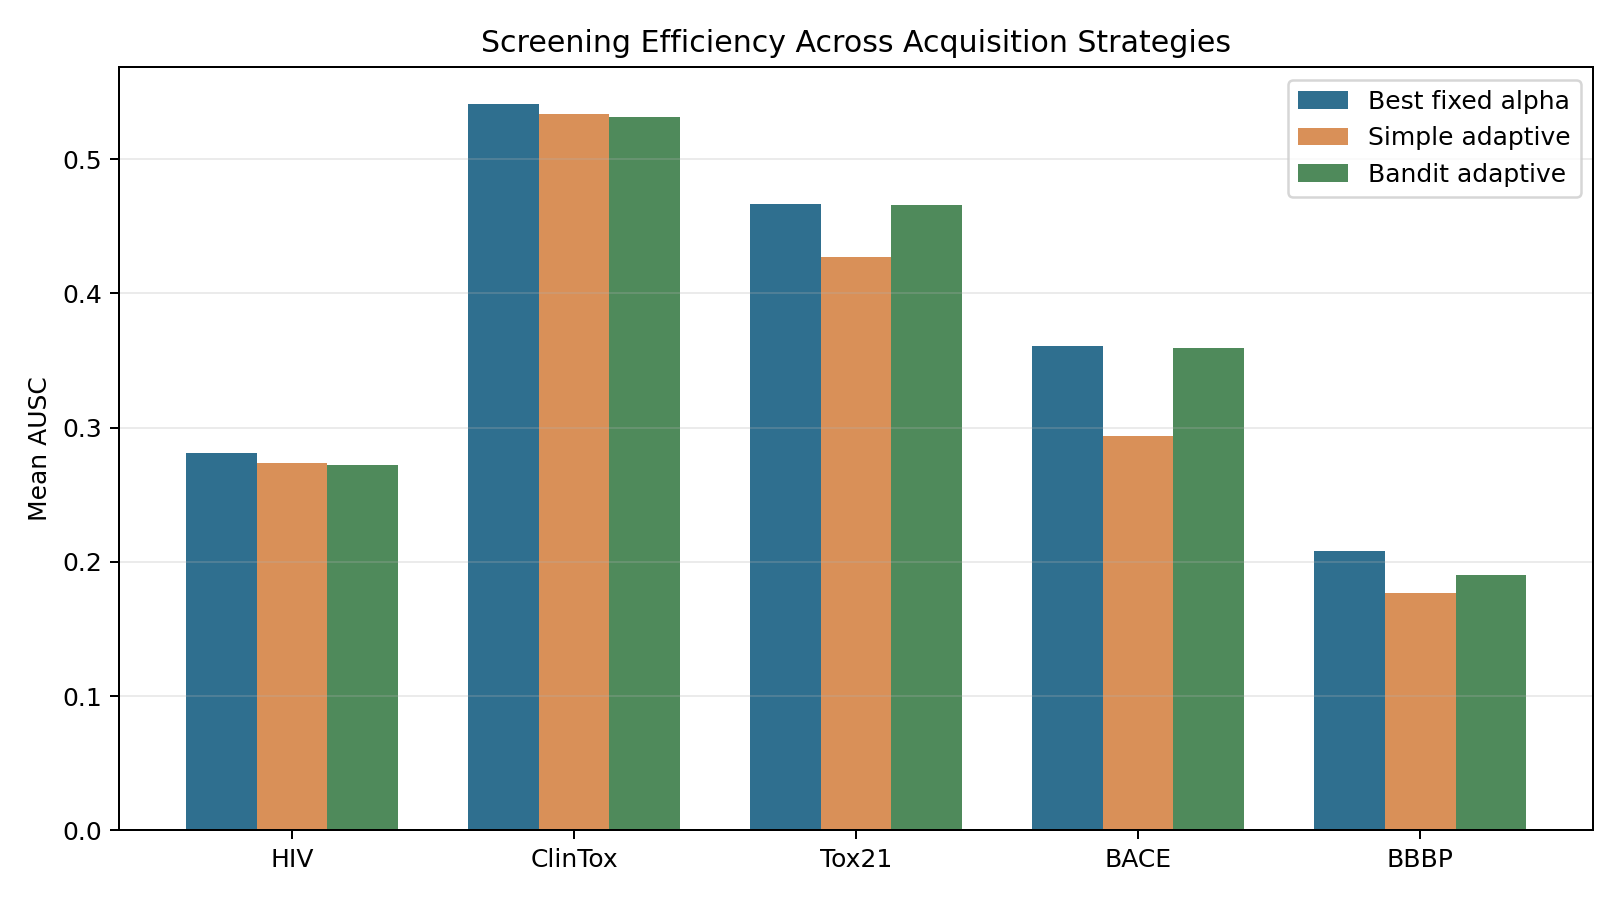
\includegraphics[width=0.86\linewidth]{figures/strategy_ausc_comparison.png}
\caption{AUSC comparison between best fixed alpha, simple adaptive alpha, and bandit adaptive alpha. Bandit alpha nearly matches the best fixed alpha on BACE and Tox21.}
\label{fig:ausc-comparison}
\end{figure}

\begin{figure}[H]
\centering
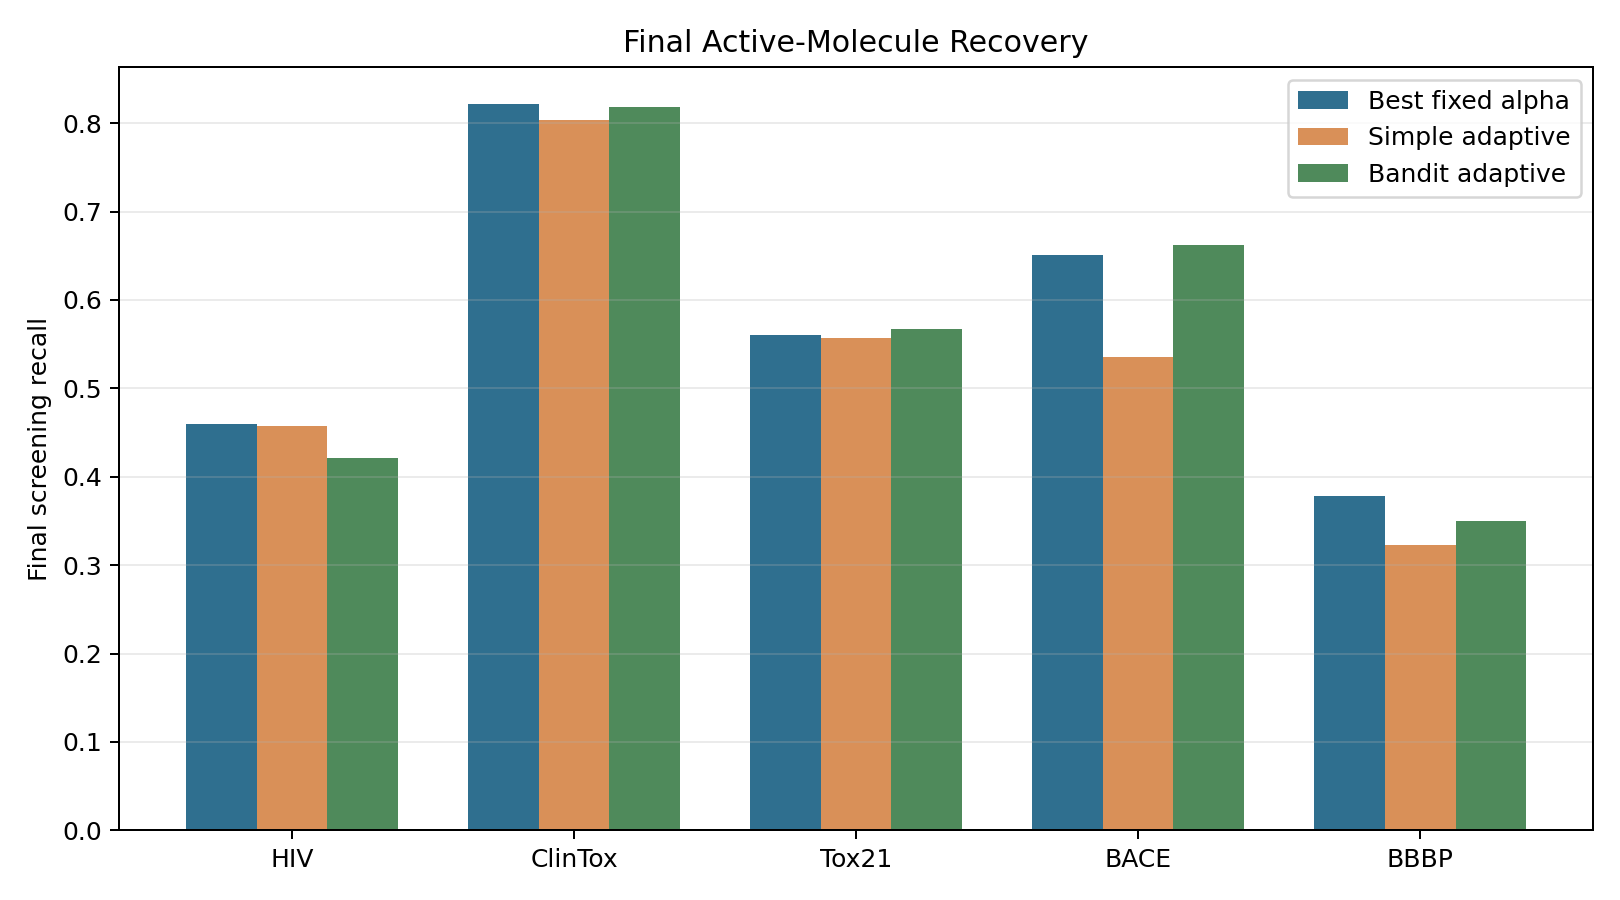
\includegraphics[width=0.86\linewidth]{figures/strategy_recall_comparison.png}
\caption{Final screening recall comparison. Bandit alpha achieves higher final recall than the best fixed alpha on BACE and Tox21.}
\label{fig:recall-comparison}
\end{figure}

\begin{figure}[H]
\centering
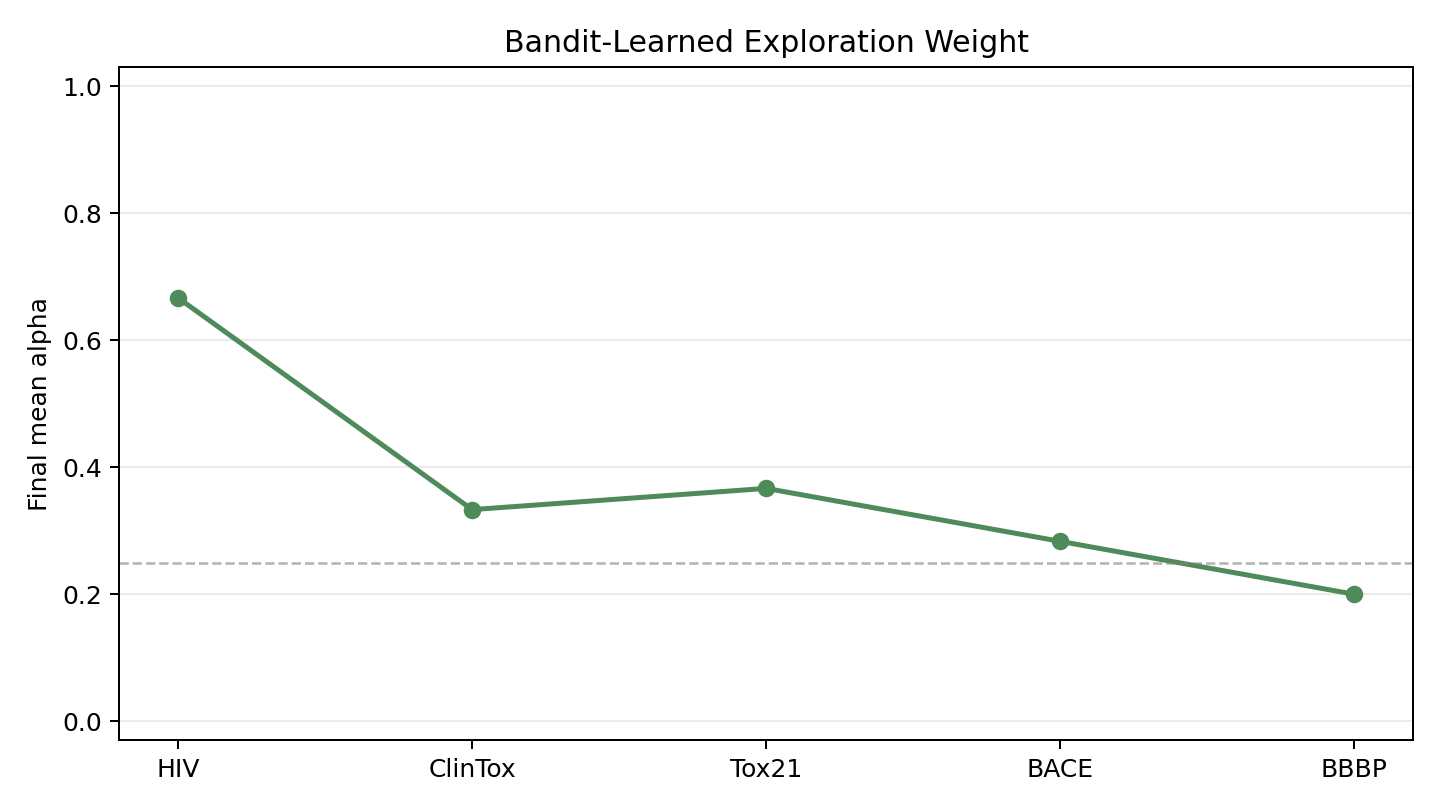
\includegraphics[width=0.76\linewidth]{figures/bandit_final_alpha.png}
\caption{Final mean alpha selected by the bandit adaptive strategy. The learned exploration weight differs across datasets.}
\label{fig:bandit-alpha}
\end{figure}

\subsection{Cluster-Weighted Bandit Results}

Cluster-weighted bandit acquisition adds structural diversity pressure to the bandit method. Table~\ref{tab:cluster-bandit} shows that this diversity mechanism creates a clear tradeoff. It improves final recall on HIV and BBBP relative to standard bandit acquisition, but it reduces AUSC on most datasets. This means that cluster diversity is useful as a secondary screening objective, but it should not dominate the hit-seeking score.

\begin{table}[H]
\centering
\caption{Cluster-weighted bandit results with cluster penalty $\lambda=0.03$.}
\label{tab:cluster-bandit}
\resizebox{\linewidth}{!}{%
\begin{tabular}{lrrrrrr}
\toprule
Dataset & Bandit AUSC & Bandit recall & Cluster AUSC & Cluster recall & $\Delta$ AUSC & $\Delta$ recall \\
\midrule
HIV & 0.2720 & 0.4214 & 0.2694 & 0.4476 & -0.0026 & 0.0262 \\
ClinTox CT\_TOX & 0.5316 & 0.8185 & 0.4957 & 0.7852 & -0.0359 & -0.0333 \\
Tox21 NR-AR & 0.4660 & 0.5667 & 0.4513 & 0.5529 & -0.0147 & -0.0138 \\
BACE & 0.3590 & 0.6624 & 0.3537 & 0.6480 & -0.0053 & -0.0144 \\
BBBP & 0.1901 & 0.3503 & 0.1898 & 0.3543 & -0.0003 & 0.0040 \\
\bottomrule
\end{tabular}
}
\end{table}

\begin{figure}[H]
\centering
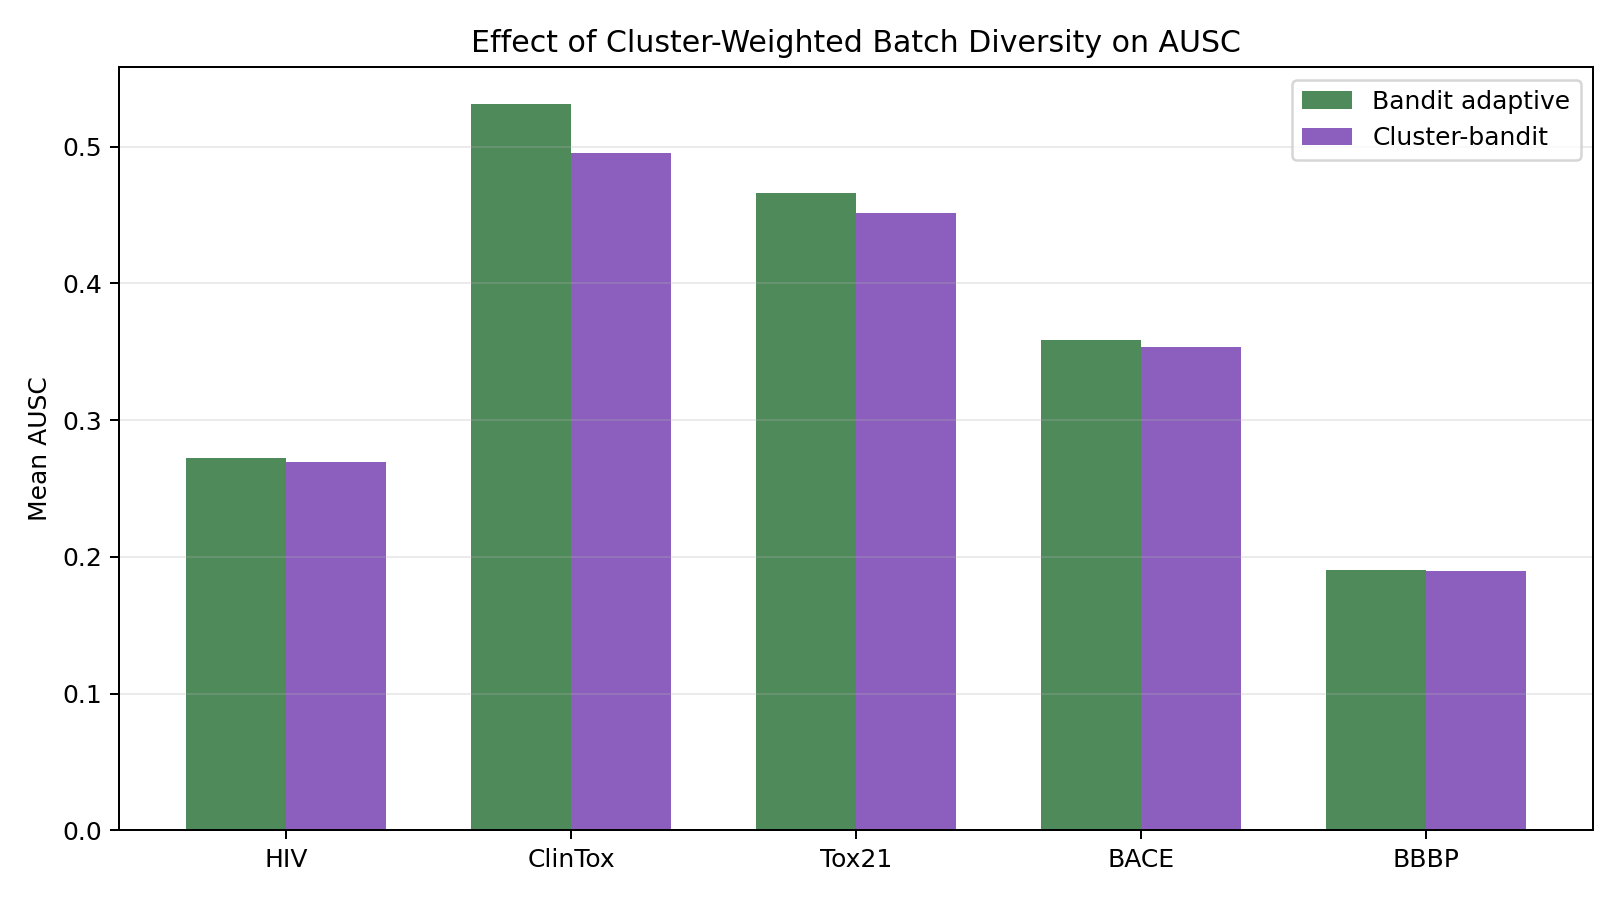
\includegraphics[width=0.86\linewidth]{figures/cluster_bandit_ausc_comparison.png}
\caption{AUSC comparison between standard bandit acquisition and cluster-weighted bandit acquisition. Cluster diversity slightly reduces AUSC in this setting.}
\label{fig:cluster-ausc}
\end{figure}

\begin{figure}[H]
\centering
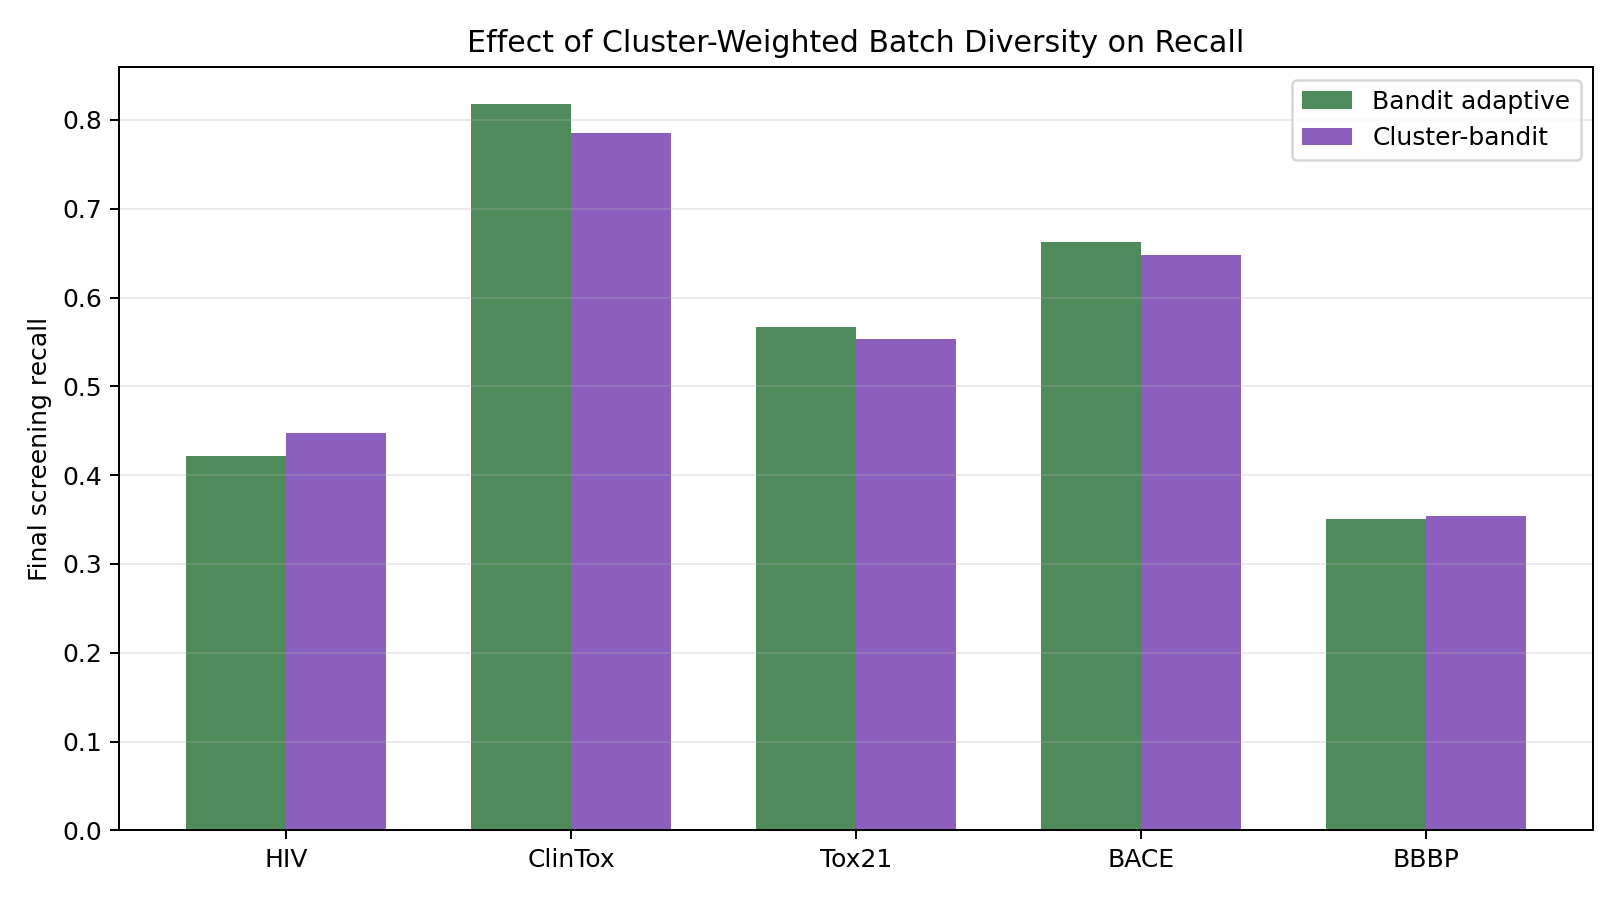
\includegraphics[width=0.86\linewidth]{figures/cluster_bandit_recall_comparison.png}
\caption{Final recall comparison between standard bandit acquisition and cluster-weighted bandit acquisition. Cluster diversity improves final recall on HIV and BBBP, but not uniformly across datasets.}
\label{fig:cluster-recall}
\end{figure}

\section{Discussion}

The results support three main conclusions.

\paragraph{First, virtual screening favors objective-aligned acquisition.}
Pure exploitation is a strong baseline because it directly targets molecules predicted to be active. This confirms that the problem should not be framed as simply training a better classifier or querying the most uncertain molecule.

\paragraph{Second, the optimal exploration weight is dataset-dependent.}
No single fixed alpha dominates across all datasets. HIV and BBBP prefer $\alpha=0$, while Tox21 and BACE prefer mild exploration. ClinTox has the best AUSC at $\alpha=0.5$, although the margin over more exploitative settings is small.

\paragraph{Third, bandit adaptation is a stronger adaptive strategy than the simple update rule.}
The simple adaptive rule can move alpha in the wrong direction, especially when recent batch hit rate is noisy. The UCB bandit method is more robust because it compares several candidate alpha values online. It does not always beat the best fixed alpha selected with hindsight, but it is competitive and gives especially strong results on BACE and Tox21.

\paragraph{Fourth, cluster diversity creates a hit-recovery tradeoff.}
Cluster-weighted bandit acquisition is motivated by the fact that drug discovery often values structurally diverse hits, not just many hits. However, the current cluster penalty reduces AUSC on most datasets. This suggests that diversity-aware acquisition is promising, but the diversity weight should be tuned or adapted online rather than fixed.

\section{Conclusion}

This study reframes active learning for ligand-based virtual screening as a dataset-dependent exploration-exploitation problem. Across five datasets, the best acquisition strategy is usually exploitative or mildly exploratory rather than pure uncertainty-driven. The bandit adaptive alpha method provides a practical way to learn the exploration weight online. It improves over the simple adaptive rule and nearly matches the hindsight-selected best fixed alpha on several datasets. The cluster-weighted extension adds structural diversity, but also reveals a tradeoff between diverse batch selection and fast active-molecule recovery. A natural next step is to adapt both the exploration weight $\alpha$ and the diversity penalty $\lambda$ online.

\end{document}
